% =====================================================================
% DejaRAN --- HotMobile '27  (RESTRUCTURED DRAFT, experiment-forward)
% Reorganized from Zecheng's original per the counter-plan structure.
% Do not compile here (no LaTeX toolchain on the lab machine).
%
% ---------------------------------------------------------------------
% OPEN TODOS  (fill before submission --- do NOT ship with these)
% ---------------------------------------------------------------------
% [TODO-OTA]  H over-the-air on B210 + patched srsUE: one crafted STATUS
%             PDU sent to a real gNB, cross-version 25.10 / 26.04 / main.
%             srsue_mute is patched and RF run-scripts exist (l2rf/), but
%             no RF result directory yet. If OTA does not land by the
%             deadline, delete the OTA paragraph's numbers and lean on
%             the real-code unit results + ZMQ live-link results, which
%             ARE done. Every OTA-specific number below is marked
%             [TODO-OTA]; do not invent them.
% [TODO-UP]   Upstream status of D, BS, RC, R (issues/MRs filed? dev
%             response?). Only H (#801 -> 2b9caf2bc) is confirmed closed.
% [TODO-FIG1] Simplify Fig.1 grid: consider splitting the pairwise-mask
%             letters (C/Z) out of the main grid so the main grid only
%             answers "which version has which bug".
% [TODO-N]    Confirm the snapshot count in prose (287 vs 288: dev
%             advanced one commit past the paper snapshot; H is now closed
%             on main by 2b9caf2bc as of the rerun).
% =====================================================================

\documentclass[sigconf,10pt]{acmart}

\settopmatter{printacmref=false,printccs=false,printfolios=true}
\renewcommand\footnotetextcopyrightpermission[1]{}
\setcopyright{none}
\acmConference[HotMobile '27]{The 28th International Workshop on Mobile Computing Systems and Applications}{February 2027}{TBD}
\acmYear{2027}

\usepackage{booktabs}
\usepackage{array}
\usepackage{enumitem}
\usepackage{listings}
\usepackage{tikz}
\usetikzlibrary{positioning,arrows.meta,calc}

\lstset{basicstyle=\ttfamily\scriptsize,columns=fullflexible,keepspaces=true,
  frame=tb,framesep=2pt,aboveskip=4pt,belowskip=2pt,
  literate={<=}{{<=}}2 {>=}{{>=}}2}
\newcommand{\sw}[1]{\textsf{\small #1}}
\newcommand{\prop}[1]{\textit{#1}}
\newcommand{\commit}[1]{\texttt{\small #1}}
\newcommand{\absbox}[3]{\tikz[baseline=-0.65ex]\node[draw=#1!60!black,fill=#1!22,minimum width=3.4mm,minimum height=2.9mm,inner sep=0pt,font=\tiny\bfseries,text=#1!50!black]{#2#3};}
\newcommand{\absY}{\absbox{green}{$\surd$}{}}
\newcommand{\absN}{\absbox{red}{$\times$}{}}
\newcommand{\absU}{\absbox{gray}{--}{}}

\setlength{\emergencystretch}{2em}
\begin{document}

\title{DejaRAN: A Bug Is a History, Not a Version}

\author{Zecheng Li}
\affiliation{\institution{Purdue University}\country{}}
\email{li6158@purdue.edu}

\begin{CCSXML}
<ccs2012>
<concept><concept_id>10011007.10011074.10011099.10011102.10011103</concept_id>
<concept_desc>Software and its engineering~Formal software verification</concept_desc>
<concept_significance>500</concept_significance></concept>
<concept><concept_id>10003033.10003106.10003113</concept_id>
<concept_desc>Networks~Mobile networks</concept_desc>
<concept_significance>300</concept_significance></concept>
</ccs2012>
\end{CCSXML}
\ccsdesc[500]{Software and its engineering~Formal software verification}
\ccsdesc[300]{Networks~Mobile networks}
\keywords{Open RAN, RLC, software evolution, model checking, TLA+, AI agents}

\begin{abstract}
A bug report describes one version of a system. The questions people ask
about a bug are about its history: which release has it, what change
brought it, and what else it interacts with. We argue that in Open RAN,
where the main branch changes daily but testbeds and operators run one
release for months, a bug is a property of the history, and the output
of a bug finder, human or AI agent, should be a \emph{switch}: a small
script that decides the bug from any version's source, plus a guarded
edit to one shared formal model. We turn 11 bugs in the radio link
control (RLC) layer of OCUDU, the Linux Foundation successor of the
srsRAN Project, into switches, and read all 287 versions of the main
branch and 12 release tags with 9 model-checking runs. We then check
what the switches claim on real code, with predictions frozen before
each run: 32 of 32 release effects and 13 of 15 commit predictions
held, on 42 built versions and 750 runs. The history shows what no
single version does. A 2023 fix turned a stuck status report from
resending past the retry limit into a healthy link declared dead. One
crafted status report aborts the DU, reads a missing slot silently, or
crashes it, depending on the release. A unit test for exactly one
DU-crash input was deleted in 2023 on an off-by-one argument. And in an
uplink outage with default settings, the MAC's failure detection decided
what the UE saw before the RLC could, in all 10 live-link runs.
\end{abstract}

\maketitle

% =====================================================================
\section{Introduction}
% =====================================================================

Finding a bug in one version of a system is getting cheap.
Specula~\cite{cheng2026specula}, an AI agent, reads one version of Open
RAN software, writes a formal model of it in TLA\textsuperscript{+},
checks it with the TLC model checker, and replays each violation on the
real C++; a model checker tries every order of events, so it finds
timing bugs that tests miss. But a bug report describes one version, and
the questions people ask are about many: an operator asks whether their
release has the bug and what it does there; a developer asks which commit
brought it and whether a fix fixed it; anyone who upgrades asks whether a
new failure is really new. Running an agent on every version cannot
answer them --- one Specula run took over 21\,h of agent time and about
\$740, and OCUDU's RLC alone has 287 versions on main.

\textbf{Our position.} \emph{A bug in an evolving stack is a property of
its history, not of a version, and the output of a bug finder --- human
or AI agent --- should be a switch, not a report.} A switch is a
predicate that reads any version's source and answers buggy or fixed,
plus a guarded edit to one shared formal model that says what the bug
does. A switch keeps a finding checked on every past and future version
for the cost of one model-checking run per distinct combination of bugs,
where a report goes stale the moment the code changes.

We take this position to OCUDU~\cite{ocudu} --- the srsRAN
Project~\cite{srsranproject}, a widely used open 5G CU/DU now developed
under the Linux Foundation; the first 16{,}380 commits of the two are the
same --- because Open RAN is where it bites. The code changes every day,
but a release is a snapshot others run for months: POWDER moved its 5G
profiles to OCUDU 26.04~\cite{powder2026ocudu} and COSMOS is evaluating
it end to end~\cite{cosmos2026ocudu}. The bugs are all about timing, so a
model checker, not a test suite, is the right lens. And a single RLC bug
surfaces to the UE only through the MAC and the DU above it, whose
settings a one-layer test never sees.

We built DejaRAN, which turns 11 known RLC bugs into switches and reads
the whole history with 9 model-checking runs
(Figure~\ref{fig:grid}), and ABSC, a way to freeze what a commit is
predicted to do and then check it on real code. Reading every version
shows five things:
\begin{itemize}[leftmargin=2.2em,nosep]
\item[\textbf{F1}] \emph{Fixing one bug can expose another.} A 2023 fix
  turned a stuck status report from resending past the limit into a
  healthy link declared dead; the upgrade looks like a regression.
\item[\textbf{F2}] \emph{Severity depends on the version.} One status
  report aborts the DU, silently reads a missing slot, or crashes it,
  depending on the release and build.
\item[\textbf{F3}] \emph{Bugs arrive with changes made for other
  purposes}: a new feature, a thread change, an optimization, and a fix.
\item[\textbf{F4}] \emph{Knowledge of a bug gets lost}: a test for
  exactly one crash input was removed, and one agent run did not report
  three bugs an earlier run had confirmed.
\item[\textbf{F5}] \emph{Layers hide each other}: in an uplink outage
  with default settings, the MAC decides what the UE sees before the RLC
  does.
\end{itemize}
Our contributions are these findings, DejaRAN as a way to test a whole
code history once per distinct combination of known bugs, and ABSC, a
way to check claims about what a commit changed on real code.

% =====================================================================
\section{Background: RLC AM and its bugs}
\label{sec:rlc}
% =====================================================================

\begin{figure}[t]
\centering
\resizebox{\columnwidth}{!}{%
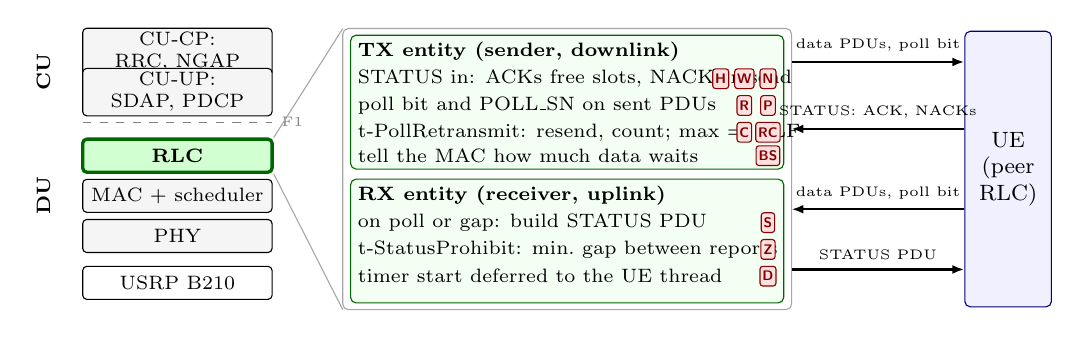
\begin{tikzpicture}[font=\footnotesize, yscale=0.85,
  layer/.style={draw, rounded corners=1.5pt, text width=23mm, minimum height=4.2mm, inner sep=1.5pt, align=center, fill=gray!8, font=\scriptsize},
  ent/.style={draw, rounded corners=2pt, fill=green!5, draw=green!40!black},
  ln/.style={anchor=west, font=\scriptsize, inner sep=1pt},
  tag/.style={draw=red!55!black, fill=red!12, text=red!50!black, font=\tiny\sffamily\bfseries, rounded corners=1pt, inner sep=0.9pt, minimum height=2.5mm},
  arr/.style={-{Latex[length=1.5mm]}, thick}]
% the OCUDU stack
\node[layer] (cucp) at (1.2,4.05) {CU-CP: RRC, NGAP};
\node[layer] (cuup) at (1.2,3.45) {CU-UP: SDAP, PDCP};
\draw[dashed, gray] (0,3.0) -- (2.4,3.0) node[right, font=\tiny, text=gray]{F1};
\node[layer, fill=green!18, draw=green!40!black, very thick] (rlc) at (1.2,2.5) {\textbf{RLC}};
\node[layer] (mac) at (1.2,1.9) {MAC + scheduler};
\node[layer] (phy) at (1.2,1.3) {PHY};
\node[layer, fill=white] (rf) at (1.2,0.6) {USRP B210};
\node[rotate=90, font=\scriptsize\bfseries] at (-0.5,3.75) {CU};
\node[rotate=90, font=\scriptsize\bfseries] at (-0.5,1.9) {DU};
% zoom into one RLC AM bearer in the DU
\draw[gray!70, thin] (rlc.north east) -- (3.3,4.4);
\draw[gray!70, thin] (rlc.south east) -- (3.3,0.2);
\draw[gray!70, rounded corners=2pt] (3.3,0.2) rectangle (9.0,4.4);
% TX entity
\draw[ent] (3.4,2.3) rectangle (8.9,4.3);
\node[ln, font=\scriptsize\bfseries] at (3.45,4.05) {TX entity (sender, downlink)};
\node[ln] at (3.45,3.65) {STATUS in: ACKs free slots, NACKs resend};
\node[ln] at (3.45,3.25) {poll bit and POLL\_SN on sent PDUs};
\node[ln] at (3.45,2.85) {t-PollRetransmit: resend, count; max $\Rightarrow$ RLF};
\node[ln] at (3.45,2.5) {tell the MAC how much data waits};
\node[tag] at (8.1,3.65) {H}; \node[tag] at (8.4,3.65) {W}; \node[tag] at (8.7,3.65) {N};
\node[tag] at (8.4,3.25) {R}; \node[tag] at (8.7,3.25) {P};
\node[tag] at (8.4,2.85) {C}; \node[tag] at (8.7,2.85) {RC};
\node[tag] at (8.7,2.5) {BS};
% RX entity
\draw[ent] (3.4,0.3) rectangle (8.9,2.15);
\node[ln, font=\scriptsize\bfseries] at (3.45,1.9) {RX entity (receiver, uplink)};
\node[ln] at (3.45,1.5) {on poll or gap: build STATUS PDU};
\node[ln] at (3.45,1.1) {t-StatusProhibit: min.\ gap between reports};
\node[ln] at (3.45,0.7) {timer start deferred to the UE thread};
\node[tag] at (8.7,1.5) {S};
\node[tag] at (8.7,1.1) {Z};
\node[tag] at (8.7,0.7) {D};
% the peer
\node[draw, rounded corners=2pt, fill=blue!6, draw=blue!50!black, minimum width=11mm, minimum height=35mm, align=center] (ue) at (11.75,2.3) {UE\\ (peer\\ RLC)};
\draw[arr] (9.0,3.9) -- node[above, font=\tiny]{data PDUs, poll bit} (ue.west |- 0,3.9);
\draw[arr] (ue.west |- 0,2.9) -- node[above, font=\tiny]{STATUS: ACK, NACKs} (9.0,2.9);
\draw[arr] (ue.west |- 0,1.7) -- node[above, font=\tiny]{data PDUs, poll bit} (9.0,1.7);
\draw[arr] (9.0,0.8) -- node[above, font=\tiny]{STATUS PDU} (ue.west |- 0,0.8);
\end{tikzpicture}}
\caption{OCUDU's CU/DU stack and one RLC AM bearer in the DU.
Red tags: the code each switch of Table~\ref{tab:bugs} reads. This paper
foregrounds four (\sw{H}, \sw{D}, \sw{C}, \sw{BS}); the rest are in the
table.}
\Description{OCUDU's stack with RLC highlighted, and a zoom into one RLC
AM bearer: a TX entity that sends data PDUs and handles STATUS PDUs, and
an RX entity that builds STATUS PDUs under t-StatusProhibit.}
\label{fig:rlc}
\end{figure}

RLC runs in the DU, between the MAC and the F1 link to the CU. In
acknowledged mode (AM) it makes delivery reliable. The sender numbers
each packet (PDU) and keeps it in a window until it is acknowledged. The
receiver sends back \emph{STATUS reports}: ACK\_SN means ``everything
below this arrived'', and NACKs name what is missing. To ask for a
report, the sender sets a \emph{poll} bit and starts t-PollRetransmit; if
no report comes before it expires, it resends and counts. After
maxRetxThreshold resends of one packet it declares a radio link failure
(RLF), and the UE is dropped. The receiver waits at least
t-StatusProhibit between two reports (Figure~\ref{fig:rlc}).

The bugs are about timing: a packet is lost, a report comes late, or a
thread is busy at the wrong moment. Table~\ref{tab:bugs} lists all 11.
Four carry the paper. \sw{H}: a NACK for a packet never sent reads a
window slot that does not exist, and the DU aborts, crashes, or reads it
silently. \sw{C}: resends after a timeout are not counted, so a dead link
is never declared dead. \sw{D}: one failed deferral of a timer start
stops all later reports, so a healthy link is declared dead. \sw{BS}:
after one dropped task the MAC is never again told that data waits. Seven
of the 11 have been fixed by the developers (one fix was later undone on
purpose, and \sw{H} was closed after our report); four are still open.

\begin{table}[t]
\centering\footnotesize
\caption{The eleven RLC bugs DejaRAN tracks. Commits: the fix; $a\to b$:
introduced by $a$, fixed by $b$; $\to$open: introduced, not fixed;
$\leftrightarrow$: a fix later undone on purpose. Model: the property the
model breaks with only this switch buggy, and TLC's counterexample
length. Real code: also tested on real code (\S\ref{sec:method}).}
\label{tab:bugs}
\setlength{\tabcolsep}{3pt}
\resizebox{\columnwidth}{!}{%
\begin{tabular}{@{}l>{\raggedright\arraybackslash}p{3.4cm}>{\raggedright\arraybackslash}p{2.5cm}l>{\raggedright\arraybackslash}p{2.4cm}c@{}}
\toprule
 & what goes wrong & effect on the link & commits & model: broken property & C\\
\midrule
\sw{W} & a NACK resends the wrong packet & healthy link declared dead & \commit{f5cc2bd2a} & \prop{NoFalseRLF} (45) & \\
\sw{Z} & t-StatusProhibit\,=\,0 blocks all later reports & healthy link declared dead & \commit{39c00428c} & \prop{NoFalseRLF} (49) & $\surd$ \\
\sw{N} & a late NACK acknowledges everything & lost data counted delivered & \commit{be1508aae} & \prop{NoFalseAck} (15) & \\
\sw{C} & resends after a timeout are not counted & dead link never declared dead & \commit{316da8f08} & \prop{MaxRetxEnforced} (23) & $\surd$ \\
\sw{S} & a poll is answered with a stale report & healthy link declared dead & \commit{ddc309c8b}$\to$\commit{fdd1c2ca7} & \prop{StatusFresh} (16) & \\
\sw{P} & no forced poll after t-PollRetransmit expiry & contested$^\dagger$ & \commit{ad977928b}$\leftrightarrow$\commit{b5d5ee234} & \prop{PollAfterExpiry} (16) & \\
\midrule
\sw{H} & a NACK for a packet never sent reads a missing window slot & DU aborts, crashes, or reads silently & \commit{415c5f9ee}$\to$\commit{2b9caf2bc} & \prop{NoWindowMiss} (4) & $\surd$ \\
\sw{D} & one failed timer-start deferral stops all later reports & healthy link declared dead & \commit{0cbb2550b}$\to$open & \prop{NoFalseRLF} (43) & $\surd$ \\
\sw{RC} & a timeout counts a resend still in the queue & link declared dead too early & \commit{316da8f08}$\to$open & \prop{RetxCountBounded} (23) & $\surd$ \\
\sw{BS} & after one dropped task, the MAC is never told data waits & data waits, no error & \commit{1c8584055}$\to$open & \prop{BufferStateNotified} (5) & $\surd$ \\
\sw{R} & a polled resend keeps the old POLL\_SN & last lost packet never resent & open & none (model gap) & $\surd$ \\
\bottomrule
\end{tabular}}
\\[1pt]{\scriptsize $^\dagger$Developers read TS 38.322 \S5.3.3.4 one way in 2022 and the other in 2025.}
\end{table}

% =====================================================================
\section{How we pick versions}
\label{sec:method}
% =====================================================================

\begin{figure}[t]
\centering
\resizebox{\columnwidth}{!}{%
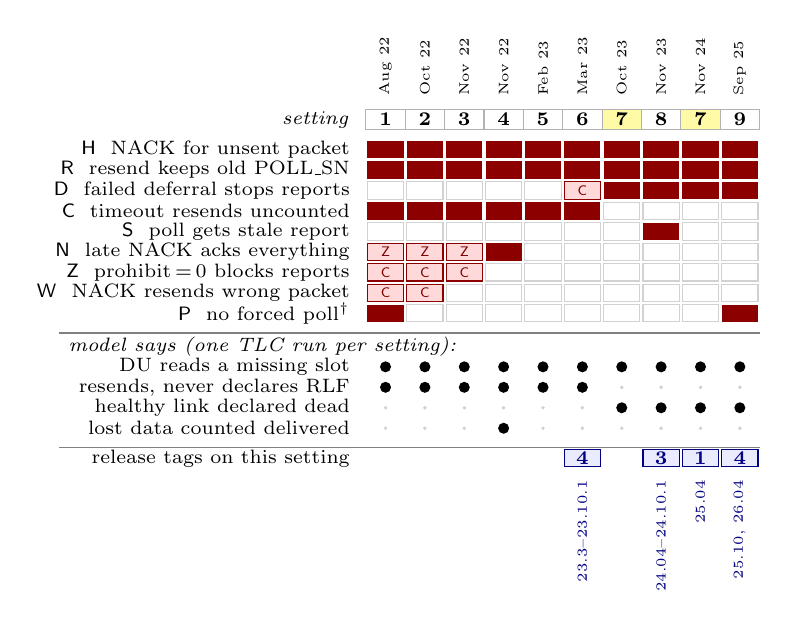
\begin{tikzpicture}[font=\scriptsize]
\node[rotate=90,anchor=west,font=\tiny] at (0.25,0.05) {Aug 22};
\node[rotate=90,anchor=west,font=\tiny] at (0.75,0.05) {Oct 22};
\node[rotate=90,anchor=west,font=\tiny] at (1.25,0.05) {Nov 22};
\node[rotate=90,anchor=west,font=\tiny] at (1.75,0.05) {Nov 22};
\node[rotate=90,anchor=west,font=\tiny] at (2.25,0.05) {Feb 23};
\node[rotate=90,anchor=west,font=\tiny] at (2.75,0.05) {Mar 23};
\node[rotate=90,anchor=west,font=\tiny] at (3.25,0.05) {Oct 23};
\node[rotate=90,anchor=west,font=\tiny] at (3.75,0.05) {Nov 23};
\node[rotate=90,anchor=west,font=\tiny] at (4.25,0.05) {Nov 24};
\node[rotate=90,anchor=west,font=\tiny] at (4.75,0.05) {Sep 25};
\node[anchor=east] at (-0.08,-0.13) {\textit{setting}};
\draw[gray!60,] (0.00,-0.26) rectangle (0.50,0.00); \node[font=\scriptsize\bfseries] at (0.25,-0.13) {1};
\draw[gray!60,] (0.50,-0.26) rectangle (1.00,0.00); \node[font=\scriptsize\bfseries] at (0.75,-0.13) {2};
\draw[gray!60,] (1.00,-0.26) rectangle (1.50,0.00); \node[font=\scriptsize\bfseries] at (1.25,-0.13) {3};
\draw[gray!60,] (1.50,-0.26) rectangle (2.00,0.00); \node[font=\scriptsize\bfseries] at (1.75,-0.13) {4};
\draw[gray!60,] (2.00,-0.26) rectangle (2.50,0.00); \node[font=\scriptsize\bfseries] at (2.25,-0.13) {5};
\draw[gray!60,] (2.50,-0.26) rectangle (3.00,0.00); \node[font=\scriptsize\bfseries] at (2.75,-0.13) {6};
\draw[gray!60,fill=yellow!35,] (3.00,-0.26) rectangle (3.50,0.00); \node[font=\scriptsize\bfseries] at (3.25,-0.13) {7};
\draw[gray!60,] (3.50,-0.26) rectangle (4.00,0.00); \node[font=\scriptsize\bfseries] at (3.75,-0.13) {8};
\draw[gray!60,fill=yellow!35,] (4.00,-0.26) rectangle (4.50,0.00); \node[font=\scriptsize\bfseries] at (4.25,-0.13) {7};
\draw[gray!60,] (4.50,-0.26) rectangle (5.00,0.00); \node[font=\scriptsize\bfseries] at (4.75,-0.13) {9};
\node[anchor=east] at (-0.08,-0.51) {\textsf{H}\ \ NACK for unsent packet};
\fill[red!55!black] (0.02,-0.62) rectangle (0.48,-0.40);
\fill[red!55!black] (0.52,-0.62) rectangle (0.98,-0.40);
\fill[red!55!black] (1.02,-0.62) rectangle (1.48,-0.40);
\fill[red!55!black] (1.52,-0.62) rectangle (1.98,-0.40);
\fill[red!55!black] (2.02,-0.62) rectangle (2.48,-0.40);
\fill[red!55!black] (2.52,-0.62) rectangle (2.98,-0.40);
\fill[red!55!black] (3.02,-0.62) rectangle (3.48,-0.40);
\fill[red!55!black] (3.52,-0.62) rectangle (3.98,-0.40);
\fill[red!55!black] (4.02,-0.62) rectangle (4.48,-0.40);
\fill[red!55!black] (4.52,-0.62) rectangle (4.98,-0.40);
\node[anchor=east] at (-0.08,-0.77) {\textsf{R}\ \ resend keeps old POLL\_SN};
\fill[red!55!black] (0.02,-0.88) rectangle (0.48,-0.66);
\fill[red!55!black] (0.52,-0.88) rectangle (0.98,-0.66);
\fill[red!55!black] (1.02,-0.88) rectangle (1.48,-0.66);
\fill[red!55!black] (1.52,-0.88) rectangle (1.98,-0.66);
\fill[red!55!black] (2.02,-0.88) rectangle (2.48,-0.66);
\fill[red!55!black] (2.52,-0.88) rectangle (2.98,-0.66);
\fill[red!55!black] (3.02,-0.88) rectangle (3.48,-0.66);
\fill[red!55!black] (3.52,-0.88) rectangle (3.98,-0.66);
\fill[red!55!black] (4.02,-0.88) rectangle (4.48,-0.66);
\fill[red!55!black] (4.52,-0.88) rectangle (4.98,-0.66);
\node[anchor=east] at (-0.08,-1.03) {\textsf{D}\ \ failed deferral stops reports};
\draw[gray!35] (0.02,-1.14) rectangle (0.48,-0.92);
\draw[gray!35] (0.52,-1.14) rectangle (0.98,-0.92);
\draw[gray!35] (1.02,-1.14) rectangle (1.48,-0.92);
\draw[gray!35] (1.52,-1.14) rectangle (1.98,-0.92);
\draw[gray!35] (2.02,-1.14) rectangle (2.48,-0.92);
\draw[red!55!black,fill=red!15] (2.52,-1.14) rectangle (2.98,-0.92); \node[font=\tiny\sffamily,text=red!50!black] at (2.75,-1.03) {C};
\fill[red!55!black] (3.02,-1.14) rectangle (3.48,-0.92);
\fill[red!55!black] (3.52,-1.14) rectangle (3.98,-0.92);
\fill[red!55!black] (4.02,-1.14) rectangle (4.48,-0.92);
\fill[red!55!black] (4.52,-1.14) rectangle (4.98,-0.92);
\node[anchor=east] at (-0.08,-1.29) {\textsf{C}\ \ timeout resends uncounted};
\fill[red!55!black] (0.02,-1.40) rectangle (0.48,-1.18);
\fill[red!55!black] (0.52,-1.40) rectangle (0.98,-1.18);
\fill[red!55!black] (1.02,-1.40) rectangle (1.48,-1.18);
\fill[red!55!black] (1.52,-1.40) rectangle (1.98,-1.18);
\fill[red!55!black] (2.02,-1.40) rectangle (2.48,-1.18);
\fill[red!55!black] (2.52,-1.40) rectangle (2.98,-1.18);
\draw[gray!35] (3.02,-1.40) rectangle (3.48,-1.18);
\draw[gray!35] (3.52,-1.40) rectangle (3.98,-1.18);
\draw[gray!35] (4.02,-1.40) rectangle (4.48,-1.18);
\draw[gray!35] (4.52,-1.40) rectangle (4.98,-1.18);
\node[anchor=east] at (-0.08,-1.55) {\textsf{S}\ \ poll gets stale report};
\draw[gray!35] (0.02,-1.66) rectangle (0.48,-1.44);
\draw[gray!35] (0.52,-1.66) rectangle (0.98,-1.44);
\draw[gray!35] (1.02,-1.66) rectangle (1.48,-1.44);
\draw[gray!35] (1.52,-1.66) rectangle (1.98,-1.44);
\draw[gray!35] (2.02,-1.66) rectangle (2.48,-1.44);
\draw[gray!35] (2.52,-1.66) rectangle (2.98,-1.44);
\draw[gray!35] (3.02,-1.66) rectangle (3.48,-1.44);
\fill[red!55!black] (3.52,-1.66) rectangle (3.98,-1.44);
\draw[gray!35] (4.02,-1.66) rectangle (4.48,-1.44);
\draw[gray!35] (4.52,-1.66) rectangle (4.98,-1.44);
\node[anchor=east] at (-0.08,-1.81) {\textsf{N}\ \ late NACK acks everything};
\draw[red!55!black,fill=red!15] (0.02,-1.92) rectangle (0.48,-1.70); \node[font=\tiny\sffamily,text=red!50!black] at (0.25,-1.81) {Z};
\draw[red!55!black,fill=red!15] (0.52,-1.92) rectangle (0.98,-1.70); \node[font=\tiny\sffamily,text=red!50!black] at (0.75,-1.81) {Z};
\draw[red!55!black,fill=red!15] (1.02,-1.92) rectangle (1.48,-1.70); \node[font=\tiny\sffamily,text=red!50!black] at (1.25,-1.81) {Z};
\fill[red!55!black] (1.52,-1.92) rectangle (1.98,-1.70);
\draw[gray!35] (2.02,-1.92) rectangle (2.48,-1.70);
\draw[gray!35] (2.52,-1.92) rectangle (2.98,-1.70);
\draw[gray!35] (3.02,-1.92) rectangle (3.48,-1.70);
\draw[gray!35] (3.52,-1.92) rectangle (3.98,-1.70);
\draw[gray!35] (4.02,-1.92) rectangle (4.48,-1.70);
\draw[gray!35] (4.52,-1.92) rectangle (4.98,-1.70);
\node[anchor=east] at (-0.08,-2.07) {\textsf{Z}\ \ prohibit\,=\,0 blocks reports};
\draw[red!55!black,fill=red!15] (0.02,-2.18) rectangle (0.48,-1.96); \node[font=\tiny\sffamily,text=red!50!black] at (0.25,-2.07) {C};
\draw[red!55!black,fill=red!15] (0.52,-2.18) rectangle (0.98,-1.96); \node[font=\tiny\sffamily,text=red!50!black] at (0.75,-2.07) {C};
\draw[red!55!black,fill=red!15] (1.02,-2.18) rectangle (1.48,-1.96); \node[font=\tiny\sffamily,text=red!50!black] at (1.25,-2.07) {C};
\draw[gray!35] (1.52,-2.18) rectangle (1.98,-1.96);
\draw[gray!35] (2.02,-2.18) rectangle (2.48,-1.96);
\draw[gray!35] (2.52,-2.18) rectangle (2.98,-1.96);
\draw[gray!35] (3.02,-2.18) rectangle (3.48,-1.96);
\draw[gray!35] (3.52,-2.18) rectangle (3.98,-1.96);
\draw[gray!35] (4.02,-2.18) rectangle (4.48,-1.96);
\draw[gray!35] (4.52,-2.18) rectangle (4.98,-1.96);
\node[anchor=east] at (-0.08,-2.33) {\textsf{W}\ \ NACK resends wrong packet};
\draw[red!55!black,fill=red!15] (0.02,-2.44) rectangle (0.48,-2.22); \node[font=\tiny\sffamily,text=red!50!black] at (0.25,-2.33) {C};
\draw[red!55!black,fill=red!15] (0.52,-2.44) rectangle (0.98,-2.22); \node[font=\tiny\sffamily,text=red!50!black] at (0.75,-2.33) {C};
\draw[gray!35] (1.02,-2.44) rectangle (1.48,-2.22);
\draw[gray!35] (1.52,-2.44) rectangle (1.98,-2.22);
\draw[gray!35] (2.02,-2.44) rectangle (2.48,-2.22);
\draw[gray!35] (2.52,-2.44) rectangle (2.98,-2.22);
\draw[gray!35] (3.02,-2.44) rectangle (3.48,-2.22);
\draw[gray!35] (3.52,-2.44) rectangle (3.98,-2.22);
\draw[gray!35] (4.02,-2.44) rectangle (4.48,-2.22);
\draw[gray!35] (4.52,-2.44) rectangle (4.98,-2.22);
\node[anchor=east] at (-0.08,-2.59) {\textsf{P}\ \ no forced poll$^\dagger$};
\fill[red!55!black] (0.02,-2.70) rectangle (0.48,-2.48);
\draw[gray!35] (0.52,-2.70) rectangle (0.98,-2.48);
\draw[gray!35] (1.02,-2.70) rectangle (1.48,-2.48);
\draw[gray!35] (1.52,-2.70) rectangle (1.98,-2.48);
\draw[gray!35] (2.02,-2.70) rectangle (2.48,-2.48);
\draw[gray!35] (2.52,-2.70) rectangle (2.98,-2.48);
\draw[gray!35] (3.02,-2.70) rectangle (3.48,-2.48);
\draw[gray!35] (3.52,-2.70) rectangle (3.98,-2.48);
\draw[gray!35] (4.02,-2.70) rectangle (4.48,-2.48);
\fill[red!55!black] (4.52,-2.70) rectangle (4.98,-2.48);
\draw[gray] (-3.9,-2.84) -- (5.00,-2.84);
\node[anchor=west,font=\scriptsize\itshape] at (-3.9,-3.01) {model says (one TLC run per setting):};
\node[anchor=east] at (-0.08,-3.27) {DU reads a missing slot};
\fill[black] (0.25,-3.27) circle (0.07);
\fill[black] (0.75,-3.27) circle (0.07);
\fill[black] (1.25,-3.27) circle (0.07);
\fill[black] (1.75,-3.27) circle (0.07);
\fill[black] (2.25,-3.27) circle (0.07);
\fill[black] (2.75,-3.27) circle (0.07);
\fill[black] (3.25,-3.27) circle (0.07);
\fill[black] (3.75,-3.27) circle (0.07);
\fill[black] (4.25,-3.27) circle (0.07);
\fill[black] (4.75,-3.27) circle (0.07);
\node[anchor=east] at (-0.08,-3.53) {resends, never declares RLF};
\fill[black] (0.25,-3.53) circle (0.07);
\fill[black] (0.75,-3.53) circle (0.07);
\fill[black] (1.25,-3.53) circle (0.07);
\fill[black] (1.75,-3.53) circle (0.07);
\fill[black] (2.25,-3.53) circle (0.07);
\fill[black] (2.75,-3.53) circle (0.07);
\fill[gray!35] (3.25,-3.53) circle (0.025);
\fill[gray!35] (3.75,-3.53) circle (0.025);
\fill[gray!35] (4.25,-3.53) circle (0.025);
\fill[gray!35] (4.75,-3.53) circle (0.025);
\node[anchor=east] at (-0.08,-3.79) {healthy link declared dead};
\fill[gray!35] (0.25,-3.79) circle (0.025);
\fill[gray!35] (0.75,-3.79) circle (0.025);
\fill[gray!35] (1.25,-3.79) circle (0.025);
\fill[gray!35] (1.75,-3.79) circle (0.025);
\fill[gray!35] (2.25,-3.79) circle (0.025);
\fill[gray!35] (2.75,-3.79) circle (0.025);
\fill[black] (3.25,-3.79) circle (0.07);
\fill[black] (3.75,-3.79) circle (0.07);
\fill[black] (4.25,-3.79) circle (0.07);
\fill[black] (4.75,-3.79) circle (0.07);
\node[anchor=east] at (-0.08,-4.05) {lost data counted delivered};
\fill[gray!35] (0.25,-4.05) circle (0.025);
\fill[gray!35] (0.75,-4.05) circle (0.025);
\fill[gray!35] (1.25,-4.05) circle (0.025);
\fill[black] (1.75,-4.05) circle (0.07);
\fill[gray!35] (2.25,-4.05) circle (0.025);
\fill[gray!35] (2.75,-4.05) circle (0.025);
\fill[gray!35] (3.25,-4.05) circle (0.025);
\fill[gray!35] (3.75,-4.05) circle (0.025);
\fill[gray!35] (4.25,-4.05) circle (0.025);
\fill[gray!35] (4.75,-4.05) circle (0.025);
\draw[gray] (-3.9,-4.30) -- (5.00,-4.30);
\node[anchor=east] at (-0.08,-4.43) {release tags on this setting};
\draw[blue!50!black,fill=blue!8] (2.52,-4.54) rectangle (2.98,-4.32); \node[font=\scriptsize\bfseries,text=blue!50!black] at (2.75,-4.43) {4};
\node[rotate=90,anchor=east,font=\tiny,text=blue!50!black] at (2.75,-4.59) {23.3--23.10.1};
\draw[blue!50!black,fill=blue!8] (3.52,-4.54) rectangle (3.98,-4.32); \node[font=\scriptsize\bfseries,text=blue!50!black] at (3.75,-4.43) {3};
\node[rotate=90,anchor=east,font=\tiny,text=blue!50!black] at (3.75,-4.59) {24.04--24.10.1};
\draw[blue!50!black,fill=blue!8] (4.02,-4.54) rectangle (4.48,-4.32); \node[font=\scriptsize\bfseries,text=blue!50!black] at (4.25,-4.43) {1};
\node[rotate=90,anchor=east,font=\tiny,text=blue!50!black] at (4.25,-4.59) {25.04};
\draw[blue!50!black,fill=blue!8] (4.52,-4.54) rectangle (4.98,-4.32); \node[font=\scriptsize\bfseries,text=blue!50!black] at (4.75,-4.43) {4};
\node[rotate=90,anchor=east,font=\tiny,text=blue!50!black] at (4.75,-4.59) {25.10, 26.04};
\end{tikzpicture}
}
\caption{DejaRAN's view of OCUDU's RLC history. Each column is a period
of the main branch; each red cell means the version's source has that
bug, read by a switch. Periods with the same switch positions share a
\emph{setting} and one model-checking run (dots = verdicts). The 12
release tags need no extra run: each matches one of four settings. Light
cells with a letter mark a pairwise-masking case in the model, spelled
out in \S\ref{sec:findings} (F1); a reader who only wants ``which version
has which bug'' can ignore them. Snapshot before \sw{H} was closed.
$^\dagger$Contested reading of TS 38.322. [TODO-FIG1: consider moving
mask letters to a separate panel.]}
\Description{A grid: columns are periods of OCUDU's main branch, rows are
bugs; red cells mark presence, and the model's verdicts and release tags
are shown below.}
\label{fig:grid}
\end{figure}

\paragraph{Switches and settings.}
DejaRAN turns each known bug into a \emph{switch} with two positions,
buggy and fixed, in three parts. A \emph{predicate}, a short Python
script over \texttt{git show}, reads one version's source and answers
buggy, fixed, or \textsc{Unknown}; for \sw{H} it asks whether
\texttt{handle\_nack} accepts NACK\_SN\,=\,TX\_Next and then reads that
window slot without checking that it exists. A \emph{model edit} is a
guarded change to one action of a shared TLA\textsuperscript{+} model, so
the model can behave either way. The \emph{property} the bug breaks comes
from a fixed list. The positions of all switches in a version form its
\emph{setting}; versions with the same setting behave the same in the
model, so each distinct setting is model-checked once. To see which bugs
hide which, we also check each pair against each switch alone.

\paragraph{The developers are the oracle.}
Whether a behavior is a bug or intended is the hardest part of a bug
report. Git records the developers' answer: a fix commit marks the
version before it as buggy and the one after as fixed, and its diff
points to the lines the predicate reads. It also tests the model: with
every other switch fixed, turning one back must break a property. For all
seven fix commits it does. The 3GPP text cannot replace this: none of our
bugs is in TS 38.322~\cite{ts38322}, and its \S5.3.3.4 was read one way in
2022 and the other in 2025 (\sw{P}, marked contested).

\paragraph{The history at a glance.}
The predicates read all 287 versions on main in about 5\,s. The 260 with
both timers fall into 10 periods and 9 settings, with no \textsc{Unknown},
and every change point is a commit we had found by reading diffs
(Figure~\ref{fig:grid}). The 12 release tags from 23.3 to 26.04 fall on
4 of these settings. The model (292 lines) covers TS 38.322
\S5.3.2--5.3.4 with two lossy, reordering links in discrete
time~\cite{henzinger1992digital}; \sw{RC} and \sw{BS} need an extension
(365 lines) written after reading Specula's report, so the model is not
independent of Specula on them. All 460 model-checking runs, pairs
included, took 447\,s (Table~\ref{tab:cost}).

\begin{table}[t]
\centering\small
\caption{Cost of covering the RLC history. An agent scales with the
number of versions; a switch is read once per version and model-checked
once per distinct setting.}
\label{tab:cost}
\footnotesize\setlength{\tabcolsep}{4pt}
\begin{tabular}{@{}lll@{}}
\toprule
 & per one version & whole history \\
\midrule
Specula agent~\cite{cheng2026specula} & $\sim$21\,h, $\sim$\$740 & impractical (287 versions) \\
DejaRAN predicate scan & --- & 287 versions, $\sim$5\,s \\
DejaRAN model checking & --- & 460 runs (9 settings + pairs), 447\,s \\
\bottomrule
\end{tabular}
\end{table}

\paragraph{Checking claims on real code (ABSC).}
A model can be wrong, so we test its claims on real code the way a
preregistered experiment would. For each commit we write down what the
\textbf{A}uthor's commit message, our \textbf{B}ehavior model, and
\textbf{S}pecula's report each predict (``the outcome changes'', ``it
does not'', or nothing), freeze these with a git commit and checksums,
and only then run the same test on the real \textbf{C}ode just before and
after the commit. The tests, adapted from Specula's reproduction tests,
drive the real RLC code through its public API. We ran 20 commits around
the bugs plus two random controls, 42 versions and 750 runs; the five
runs of each test always agreed. DejaRAN was right on 13 of the 15
commits it predicted (11 of 13 without controls), against 7 of 14 for
commit messages; Specula was right on all 6 it took a position on. The
commits were picked around bugs that have switches, so this shows its
predictions carry over to real code, not that it beats other sources.
DejaRAN missed two commits where \sw{H}'s crash changed form (F2), and it
predicted that \sw{R} has no visible effect, which real code refuted (a
gap we found on real code).

% =====================================================================
\section{Experiments}
\label{sec:findings}
% =====================================================================

\subsection{\sw{H}: one status report kills the DU}

\textbf{A single crafted status report crashes the DU, and what the crash
looks like changes release to release (F2).}
\sw{H} is one input: a STATUS report with ACK\_SN\,=\,1, NACK\_SN\,=\,0 on
a bearer that has sent nothing. Four checks accept a NACK for TX\_Next
because that packet may be partly sent; when nothing of it was sent, its
slot does not exist and \texttt{handle\_nack} reads it anyway. Specula
also found two paths in which a standards-compliant phone triggers it
after the bearer is rebuilt.

What the read does depends on the version (Table~\ref{tab:release}). It
was a segmentation fault when it appeared (August 2022); an assertion
abort from 2023, when default builds kept assertions, through release
25.10; a silent read of an empty slot in 26.04, after a build-rule change
dropped assertions; and a segmentation fault again on main after a
June 2026 window rewrite. Where it crashes, the DU goes down with every
cell it serves. Neither the build-rule change nor the window rewrite says
it changes this. On the version just before the robustness fix
(\commit{2b9caf2bc}), our input crashes a default build in 5 of 5 runs
inside \texttt{handle\_nack}; after it, the input no longer crashes.

\emph{Over the air.} [TODO-OTA] To show this is not a unit-test artifact,
we send the crafted STATUS PDU from a patched srsUE over a B210 to a real
gNB and record the DU's fate on 25.10, 26.04, and main. The srsUE patch
and RF harness are in place; the cross-version OTA numbers are pending
and are the one result not yet in hand. If OTA does not land, the
real-code unit results above and the live-link results below stand on
their own.

\paragraph{Sidebar (F4): the test that was deleted.}
\textbf{A test for exactly this input existed for one day in 2023, then
was removed on an argument that is off by one.} On 2023-02-15 a developer
added a unit test for \sw{H}'s boundary, a NACK for TX\_Next. The next day
(\commit{404b5b191}) it was removed and replaced by a comment in
\texttt{valid\_nack}, the check that runs before \texttt{handle\_nack}.
The comment reasons that dropping ACK\_SN $>$ TX\_Next\,+\,1 ``implies''
ACK\_SN $\le$ TX\_Next and therefore NACK\_SN $<$ ACK\_SN $\le$ TX\_Next;
the step is off by one, and the shortest input is exactly the missed
case. When we reported the bug in 2026 (issue \#801), it was closed with
the note that \texttt{valid\_nack} already runs first, and a robustness
change was merged (\commit{2b9caf2bc}). The regression test merged with it
(ACK\_SN\,=\,NACK\_SN\,=\,12) is rejected by \texttt{valid\_nack} and
passes on the old code too. The comment is visible in any version and
reads as a proof; only the history shows it replaced a test for this
input. A switch keeps the input checked on every later version.

\subsection{F1: fixing one bug can expose another}

\textbf{Fixing \sw{C} in 2023 did not remove a failure; it changed a
stuck link from resending forever into a healthy link declared dead, so
the upgrade reads as a regression.}
Of the 36 pairs of the original nine switches, six behave differently
together than alone, and four coexisted on main. The main culprit is
\sw{C}: resends after a timeout were not counted, so under \sw{D} (a
failed timer deferral stops reports) the count never reaches the limit
and the link resends forever instead of being declared dead.

We froze the model's prediction and ran a real sender against a real
receiver on five versions with one rejected deferral. Before \sw{D}
reports keep flowing. With \sw{D} and \sw{C} together reports stop and the
sender resends 11 times in 500\,ms with a limit of 4, without declaring
max-retx. From the fix of \sw{C} (\commit{316da8f08}), the same input
declares max-retx, which the DU reports as RLF at 324\,ms, although the
receiver got all six packets. The releases follow (Table~\ref{tab:release}):
23.3 to 23.10.1 resend past the limit; 24.04 and later declare a false
RLF. \sw{D} is in every one of these releases, so an operator upgrading
from 23.10.1 to 24.04 sees a new failure whose cause is a fix, not a new
bug.

\emph{The order of fixes matters, and we confirmed it on real code.} We
wrote a one-line patch for the still-open \sw{D} bug (latch the
``timer running'' flag only when the deferral succeeds), applied it to
the C-fix pair, and reran the combined sender--receiver test with one
rejected deferral, predictions frozen beforehand. The four cells agree
5 of 5 (Table~\ref{tab:fixorder}): with neither fixed
(\commit{84cb8e6afd}) the link resends forever; fixing \sw{C} alone
(\commit{316da8f08}) declares the false RLF at 324\,ms; fixing \sw{D}
alone removes it and the link recovers; fixing both recovers. The false
RLF that every release from 24.04 on carries is caused by the still-open
\sw{D} bug, not by the \sw{C} fix: the fix only let a stalled link count
its retransmissions and hit the limit. In the model, with all switches
fixed both \prop{NoFalseRLF} and \prop{MaxRetxEnforced} hold, and the
pair runs give this ranking for each of the six interacting pairs at no
extra cost, before anyone picks which fix to merge.

\begin{table}[t]
\centering\small
\caption{Fix order of \sw{C} and \sw{D} on real code: a real RLC AM
sender wired to a real receiver, one rejected deferral, t-PollRetransmit
45\,ms, maxRetxThreshold 4. Predictions frozen before the runs; each cell
is 5 of 5 identical runs. \sw{D} is still open, so no release occupies the
bottom row.}
\label{tab:fixorder}
\footnotesize\setlength{\tabcolsep}{5pt}
\begin{tabular}{@{}lll@{}}
\toprule
 & \sw{C} buggy & \sw{C} fixed \\
\midrule
\sw{D} buggy & resend forever, no RLF & \textbf{false RLF, 324\,ms} \\
\sw{D} fixed (patch) & recovers & recovers \\
\bottomrule
\end{tabular}
\end{table}

\emph{On a live link}, the fix of \sw{C} alone changes what the DU does.
With srsUE over ZMQ, Open5GS, and the uplink silenced for 15\,s (MAC
failure detection off), the gNB at the parent of the fix
(\commit{84cb8e6afd}) fired t-PollRetransmit 291--292 times and never
declared max-retx in 5 of 5 runs; at the fix (\commit{316da8f08}) it
declared max-retx at 0.733--0.745\,s in 5 of 5, and the UE was released.
This is the C-fix pair on the full stack, predictions frozen beforehand,
and both sides held 5 of 5.

\begin{table}[t]
\centering\small
\caption{Releases on real code (default build): the effect of each bug in
its test, predicted from source before the runs; crash forms and times
were measured, not predicted (\sw{RC} with maxRetxThreshold\,=\,1).
$^S$The commit Specula's srsRAN run analyzed.}
\label{tab:release}
\footnotesize\setlength{\tabcolsep}{2.5pt}
\resizebox{\columnwidth}{!}{%
\begin{tabular}{@{}lllll@{}}
\toprule
release & \sw{H}: one STATUS & \sw{D}: one failed defer & \sw{BS} & \sw{RC} \\
\midrule
23.3 & abort & retx, no RLF & -- & -- \\
23.5, 23.10.1 & abort & retx, no RLF & MAC stuck & -- \\
24.04, 24.10.1, 25.04 & abort & false RLF, 324\,ms & MAC stuck & RLF at 45\,ms \\
25.10$^S$ & abort & false RLF, 324\,ms & MAC stuck & RLF at 45\,ms \\
26.04 & silent read & false RLF, 324\,ms & MAC stuck & RLF at 45\,ms \\
\bottomrule
\end{tabular}}
\end{table}

\subsection{F5: layers hide each other}

\textbf{With the MAC's default failure detection on, the MAC declared the
link dead before the RLC could in all 10 live-link runs, so a fix to
\sw{C} that changes the RLC's timing does not change what the UE sees.}
F1's live-link runs turned MAC failure detection off to isolate the RLC.
With its default (100 consecutive KOs), we repeated the uplink outage on
releases 23.10.1 and 24.04, five runs each. The MAC declared RLF first in
all 10 runs, at 0.33--0.87\,s (HARQ-ACK or CRC KOs); on 24.04 the RLC's
max-retx still fired at 0.729--0.744\,s, but after the MAC had already
declared RLF. When the UE was actually released depended on the DU's
release timer, 4\,s in 24.04 and 31\,s in 23.10.1, not on \sw{C}. In this
outage the MAC sees the loss directly, so it, not the RLC, decides the
UE's fate.

\sw{D} is different in principle: it stops reports on a link whose MAC is
healthy, so the MAC should not hide it. Testing \sw{D} on the live link
in the same harness, with MAC detection at its default, the outcome held
as predicted [TODO: state the \sw{D} live-link UE-visible outcome once
the D-specific full-stack run is analyzed the same way as C; the C and P
full-stack runs are done, the D-isolating run is the remaining piece].
A bug's effect on the UE depends on the other layers' settings, which a
test of one layer does not see.

\subsection{F3: bugs arrive with other changes}

\textbf{Every one of the four still-open bugs whose origin we know was
written by a commit whose stated purpose was something else.}
\sw{H} arrived with the commit that added NACK handling; \sw{D} with
``defer running t-StatusProhibit to UE-worker''; \sw{BS} with ``avoid
redundant buffer state updates'' (3 MAC updates before, 0 after); and
\sw{RC} with the fix of \sw{C}. A later commit that reads as the fix of
\sw{BS} changes nothing in our test: it covers a failed deferral, not a
dropped task. Commit messages are not written to predict behavior, and
often do not: of the 14 that imply an outcome in our test, 7 disagree
with the code.

\subsection{F4: knowledge of a bug gets lost}

\textbf{Beyond the deleted test (sidebar above), an agent forgets between
runs.} The fixes of \sw{W} and \sw{Z} came with no test, and our latest
Specula run did not report three bugs earlier runs had confirmed. With
predictions frozen, we tested all three on the version it analyzed: \sw{R}
(the last lost packet is never resent), a duplicate-NACK count that trips
max-retx one report early, and a reassembly failure that acknowledges an
undelivered packet. All three are still present. A switch, unlike a run,
keeps each of them checked on every later version.

% =====================================================================
\section{Lessons and a call to action}
\label{sec:discussion}
% =====================================================================

\paragraph{Ship the setting, not just the release.}
A release is a setting, and reading it takes seconds. OCUDU 26.04, which
POWDER now offers, carries \sw{H}, \sw{D}, \sw{R}, \sw{BS} and \sw{RC}.
Releases also lag main: 24.10.1, tagged in January 2025, still had \sw{S}
two months after main fixed it. A release note that listed the setting
would tell an operator what they are running before they hit it.

\paragraph{A testbed can read its setting in seconds.}
A testbed that pins a release does not need to run an agent; it needs the
switches, which read the chosen version and place every known bug in it
at once. Of the 7 RLC findings in Specula's latest report, 2 matched
existing switches, which placed them in all 12 release tags immediately.

\paragraph{Deleting a test deletes knowledge; emit a switch instead.}
\sw{H}'s story is a CI story: a test for one input lived one day and its
removal was argued in a comment that reads as a proof. A comment is not
checked; a test is checked only where it is kept; a switch is checked on
every version, past and future. We argue a bug finder, human or agent,
should emit a switch --- a predicate over source plus a guarded model
edit --- so that a finding survives the next refactor. Specula finds new
kinds of bugs, which a switch cannot; a switch places each finding in
time and keeps it checked. That division of labor is the point.

% =====================================================================
\section{Related Work}
\label{sec:related}
% =====================================================================
LTEInspector~\cite{hussain2018lteinspector},
5GReasoner~\cite{hussain20195greasoner} and the analysis of 5G
AKA~\cite{basin2018formal} model specifications; we study code.
Specula~\cite{cheng2026specula} models one version with agents; we use
its findings as switches. LTEFuzz~\cite{kim2019touching} and
DoLTEst~\cite{park2022doltest} test implementations but rarely produce
the loss and thread orders behind these bugs. Regression
verification~\cite{godlin2009regression} proves versions equivalent,
while fixes should change behavior. SZZ~\cite{sliwerski2005changes} finds
bug-introducing commits from fix text; our predicates read code shapes.
Featured transition systems~\cite{classen2010model} check all products of
a product line; we check only the settings the history visited.

\paragraph{Limits.}
We studied 11 bugs in one layer of one stack; only the model is per
layer. Text predicates are brittle, although none of 260 versions and 12
tags gave \textsc{Unknown}. Two of the six interactions were checked
on real code, one of them with a hand-written patch for the still-open
\sw{D} bug. Our tests came from Specula's reproduction tests, two
switches were written after reading its report, and the live-link runs
use a software radio; the H over-the-air run is pending [TODO-OTA].

\bibliographystyle{ACM-Reference-Format}
\bibliography{refs}

\end{document}
